\chapter{Related Work}

This section outlines key findings of related work on gender bias in MT, with a focus on the English-German (EN-DE) language pair to build the theoretical knowledge base. The research aims are to (1) define the core concept of gender bias in MT, (2) establish the relevance of the topic, (3) identify the research gap, and (4) justify technical design choices. To support this, I examine datasets, model types, and tools used in previous studies.

For the literature review I combined incremental and conceptual literature review methods, where each source led to the identification of the next. Based on this progression, I identified key concepts and used them to organize and interpret the literature, aligning with a conceptual approach. The structure followed the qualitative Information Systems framework by \citet{schryenWritingQualitativeLiterature2015} and was further informed by \citet{shresthaExploringGenderBiases2022} and \citet{savoldiDecadeGenderBias2025}, who both conducted systematic reviews on gender bias in ML and MT respectively. 

\section{Literature Search Process}

\subsection{Search Sources and Tools}
Sources were primarily searched on \href{https://scholar.google.com/}{Google Scholar} and \href{https://www.perplexity.ai/}{Perplexity}, which served as an additional search engine. Prompts and outputs from Perplexity have been saved and are included in the appendix. To organize and manage the collected sources, \href{https://www.zotero.org/}{Zotero} was used throughout the process.

\subsection{Literature Review Framing}

To answer the four research aims, I have defined the key concepts in \autoref{tab:key-concepts}. Key search terms consisted of \textit{gender bias}, \textit{machine translation}, \textit{AI}, \textit{machine learning}, \textit{German}, \textit{stereotypes}, and \textit{detection}. The focus was on literature published between 2019 and 2025 to maintain relevance and currency, while foundational and definitional works from earlier periods were selectively included. The initial search for the term \textit{gender bias in machine translation} returned over 18,000 results. Through my iterative selection process, this was narrowed down to 34 core sources.

\renewcommand{\arraystretch}{1.3}
\begin{table}[ht!]
\centering
\begin{tabularx}{\textwidth}{lX}
\toprule
\textbf{Key Concept} & \textbf{Description} \\
\midrule
Stereotypes and Biases in Society & Introduces the social foundations of bias by explaining how stereotypes form, persist, and shape expectations about gender roles. Necessary to understand why certain translation outputs may reflect or reinforce societal gender norms. \\

Machine and Algorithmic Bias & Explains how social biases can enter ML systems through data, design choices, or feedback mechanisms. Sets the groundwork for understanding how gender bias can emerge in translation models used in this thesis. \\

Gender Bias in EN-DE Translation & Focuses on the specific challenges of translating between English and German, where the lack of grammatical gender in English and its necessity in German can cause biased outputs. Defines the types of gender bias relevant to the classification task in this thesis. \\

Bias Detection Frameworks & Reviews existing methods for identifying gender bias in language data and ML outputs. Helps justify the choice of a classification approach for detecting bias in translations. \\

\bottomrule
\end{tabularx}
\caption{Key concepts relevant to this thesis}
\label{tab:key-concepts}
\end{table}

\subsection{Citation Tracking}
Backward citation searching involved reviewing references cited by selected papers, prioritizing frequently cited and foundational works relevant to gender bias in MT. Forward citation searching used Google Scholar's "cited by" function to identify newer research citing those key papers. Filtering with specific terms (e.g., \textit{German} and \textit{machine translation}) was applied during forward search to maintain focus. In addition to the main review process, supplementary sources were included as needed throughout the writing phase. These consist of contextual references, statistics, or secondary citations that support specific points but were not part of the core conceptual or methodological framework.

\subsection{Selection Criteria and Screening Process}\label{subsection:selection_criteria}
Titles and abstracts were manually screened to select relevant studies. \textbf{Inclusion criteria} required sources to specifically address gender bias in MT, provide examples or discussions of gender-related errors, or explain the significance of gender bias in this context. Sources also had to be available in full text without access restrictions. \textbf{Exclusion criteria} filtered out studies focusing on general NLP bias without a direct link to MT, non-gender biases, and highly technical papers lacking contribution to the general understanding of gender bias or that did not provide additional knowledge beyond what was already found in previously published papers. Full texts were reviewed after initial screening to confirm relevance and extract insights. Redundant sources not providing new perspectives aligned with the thesis goals were excluded.

\section{Foundations of Gender Bias in Natural Language Processing}

This section outlines why gender bias is a subject of research in the first place and where it connects to broader social and ethical questions. It first looks at early studies that brought attention to gender patterns in language technologies and raised awareness of their social impact. Understanding these origins helps explain how gender bias became a recognized problem in NLP and why it continues to be relevant today.

\subsection{Foundational studies}
The existence of gender bias in MT is well-documented. First mentions of this issue date back to over a decade ago, having been recognized by a paper by \citeauthor{schiebingerScientificResearchMust2014} in 2014. Since then, there has been a general increase in research papers focusing on this topic, especially between 2019 and 2023 \citep{savoldiDecadeGenderBias2025}.

\textbf{\citet{pratesAssessingGenderBias2019}} conducted a large-scale quantitative study using Google Translate, translating sentences such as "He/She is an engineer" from twelve gender-neutral languages into English. The study revealed a significant overrepresentation of male pronouns, particularly in STEM-related occupations. This skew was not attributable to actual gender distributions in the labor market, suggesting that the bias stemmed from imbalances in the system’s training data. The paper received widespread media coverage, which was followed by a policy change by \citeauthor{googleReducingGenderBias2018} to present both feminine and masculine official translations for ambiguous queries \citep{googleReducingGenderBias2018}, acknowledging that their model inadvertently replicated gender biases (see \autoref{fig:gt_prates_example}). 

\textbf{\citet{stanovskyEvaluatingGenderBias2019}} introduced \href{https://github.com/gabrielStanovsky/mt_gender}{WinoMT}, a challenge set designed to evaluate gender bias in translations of English sentences into eight target languages with grammatical gender. The study showed that both commercial and academic MT systems failed to preserve correct gender in non-stereotypical roles, while performing better on stereotypical ones. In line with the findings of \citeauthor{pratesAssessingGenderBias2019}, the study demonstrated a systematic preference for traditional gender roles in translations. This pattern is further supported by \textbf{\citet{choMeasuringGenderBias2019}}, who showed that occupational terms exhibit higher levels of gender bias across systems compared to other semantic categories. 

These foundational studies not only confirm the existence of systematic gender bias in MT outputs, but also lay the groundwork for subsequent research that builds upon their findings to develop more robust evaluation methods and mitigation strategies.

\subsection{Human-Centered Studies}
In addition to analyzing MT outputs directly, some studies have assessed the real-world implications of gender bias by measuring its impact on human effort. \citet{savoldiWhatHarmQuantifying2024} conducted a human-centered evaluation in which approximately 90 participants were tasked with post-editing MT outputs to ensure gender-accurate translations.

The study employed behavioral metrics such as time to edit and the number of edits, measured through human-targeted error rate, to quantify the effort required. The results showed that post-editing feminine translations required nearly twice as much time and four times the number of editing operations compared to masculine counterparts. Consequently this effort gap also translates into higher economic costs, suggesting a measurable quality-of-service disadvantage that disproportionately affects women. \citeauthor{savoldiWhatHarmQuantifying2024} concluded that current automatic bias metrics do not sufficiently capture these human-centered disparities, emphasizing the need for evaluation methods that reflect real user experience.

A comparison analysis between AI and human translations was conducted by \citet{smacchiaDoesAIReflect2024}. The study's aim was to understand if gender bias is still present in how people think in society. Their results demonstrated a consistency between the outcomes generated by the AI tools and the human survey responses, suggesting that AI tools reflect human behaviour regarding job occupations and gender distributions in society. They also identified a "converging bias", which is a tendency to maintain consistency in the output based on an initial translation. For example, if the \textit{doctor} in \textit{"The doctor arrived"} is translated with a male form, the subsequent input \textit{"The doctor then started working"} is likely to be translated as male too.

\subsection{Implications of Gender Bias in Natural Language Processing}
Although gender bias has long been a subject of study linguistically, the growth in research is driven by the increasing role NLP systems play in our everyday lives. As outlined in \autoref{section:social_and_ethical_importance_of_addressing}, this section builds on the social and ethical foundations by examining how gender bias in NLP can lead to the amplification of existing social biases \citep{rescignoGenderBiasMachine2023}.
\citet{ullmannGenderBiasMachine2022} illustrates this with an example: if a dataset predominantly associates cooking with women, the system may amplify this pattern, reinforcing the assumption that cooking is an activity exclusive to women. This not only reproduces but also strengthens a social stereotype, potentially resulting in \textbf{representational harm}, namely, the continued spread of reductive or biased portrayals of a particular gender \citep{stanczakSurveyGenderBias2021}. 

This also contributes to the invisibility of women in professions traditionally dominated by men \citep{kapplAreAllSpanish2025}. Studies show that gender bias in machine-generated text, such as children's stories or job advertisements, can \textbf{influence how young people view themselves} \citep{soundararajanInvestigatingGenderBias2024,kapplAreAllSpanish2025}. It may shape their interests, hobbies, and decisions about education and careers. This effect is especially noticeable in Science, Technology, Engineering, and Mathematics (STEM) fields \citep{pratesAssessingGenderBias2019}, where stereotypes are more deeply rooted. When job descriptions or mock interviews use gender-exclusive pronouns, women report feeling less sense of belonging, lower motivation, and weaker identification with the role \citep{godsilEffectsGenderRoles2016}. As a result, they may self-select out of the application process, reducing the pool of female talent available to employers and \textbf{reinforcing existing gender gaps in the workforce}.

On the other hand, research shows that using gender-inclusive language, e.g. "she and he" or "one", can lead to more positive reactions from women when considering job opportunities. It helps reduce stereotype threat and improves how women perceive and engage with different environments \citep{ godsilEffectsGenderRoles2016}. Hence, complying with gender-inclusive langauge may offer companies both social and competitive advantages.


\section{Sources and Manifestations of Bias}

To address a problem, one needs to understand its origins. This section outlines how societal bias transfers into data and NLP systems. It looks at different types of bias, with a focus on those that shape model behaviour and outputs.

\subsection{Human Bias Transfer}
Stereotypes and gender roles stem from historical and cultural perceptions of men's and women's societal roles, many of which are obsolete but still influential. For example, when men and women often take on different roles at work and at home, it shapes how people think about their personalities and qualities. \textbf{Correspondence bias} can emerge, where people infer attributes from observable behaviours \citep{godsilEffectsGenderRoles2016}. It is a result of the human brain's automatic categorization of stimuli when faced with incomplete information, often a quick and unconscious process. Common groupings are gender, race and age. These associations can be reinforced by popular media, such as TV and advertisements \citep{godsilEffectsGenderRoles2016}, just as much as it can be influenced by modern technology like MT tools. 

Similarly to how humans are shaped by their environemnt, ML models learn from data they are trained on. \textbf{Biases are thus reflected and reinforced in the final models} \citep{stanczakSurveyGenderBias2021,smacchiaDoesAIReflect2024}. That bias can, again, reflect back to humans and create a regressive feedback loop \citep{barclayInvestigatingMarkersDrivers2024a,shresthaExploringGenderBiases2022}. LLMs like GPT-3 were trained on hundreds of billions of words, making it practically impossible to review all of the data, therefore allowing misinformation or offensive content to be reproduced by the system.


\citet{ullmannGenderBiasMachine2022} notes that the scale of training data (e.g. 175 billion parametres for GPT-3) makes it practically impossible to review all of it, allowing misinformation or offensive content to be reproduced by the system. The author also points out that platforms like Wikipedia and Reddit are male-dominated and often contain harmful or false content, which contribute to gender bias.

\subsection{Types of Data Bias}
\citet{ullmannGenderBiasMachine2022} derived four types of data biases. 
% ullmann

% Selection Bias (Sample Bias): Occurs when training data is not representative of its intended use.
% ▪
% Label Bias: Happens when data is falsely or incorrectly annotated, often due to annotators not being representative of diverse demographics (e.g., misclassifying dialects as 'offensive').
% ▪
% Semantic Bias: Arises from associative relations in data, where a certain pronoun is more commonly linked to a profession due to high co-occurrences (e.g., 'he' and 'doctor').
% ▪
% Model Overamplification: During training, a system can overly amplify existing representations or distributions in the data, inadvertently magnifying social stereotypes (e.g., if cooking is mostly associated with women, the system might assume only women cook).

\section{Linguistic Challenges in English-German Translation}

Since this thesis focuses on EN-DE translation, it is important to understand how gender works in German. This section will explore the main linguistic features that affect gender expression in German. Then, it will review key studies that examine how these features influence bias in translation.

\subsection{Grammatical Gender}
Although both English and German originate from the Indo-European language family \citep{baldiEnglishIndoEuropeanLanguage2008}, they have different characteristcs. English does not assign grammatical gender to nouns. The article "the" is used universally, independent of what it refers to. On the contrary, German assigns one of three grammatical gendered articles to nouns: "der" (m), "die" (f) and "das" (n). The form or ending of a noun may also change depending on its grammatical gender. While English has a few gendered word pairs, such as "actor" (m) and "actress" (f), gender distinctions in German apply broadly across the entire noun system. "Der Student" refers to a male student, whereas "die Studentin" refers to a female student. Note that grammatical gender has no connection to societal or biological gender. It is a rule of the language rather than a reflection of identity. For example, the German word Mädchen (girl) is grammatically neuter and takes the article "das". This is not because the referent lacks gender, but because the suffix "-chen" automatically assigns neuter gender. This illustrates that grammatical gender in German follows structural rules, even when they contradict real-world gender associations.

\subsection{Gender-Fair Language}

\subsubsection{The Generic Masculine}  
In both singular and plural contexts, the \textit{generic masculine} refers to the default use of the masculine grammatical gender. It is commonly used in spoken German \citep{lardelliBuildingBridgesDataset2024,schmitzGermanAllProfessors2022}, although research has consistently shown that the generic masculine creates a male bias in mental representations, leading readers or listeners to think more of male than female examples \citep{sczesnyCanGenderFairLanguage2016}. Similarly, \citet{rescignoGenderBiasMachine2023} observed a predominance of masculine forms in translation outputs (approximately 90\% in Google Translate and 85–88\% in DeepL for EN-IT and EN-DE), even when the original sentences contained relatively few masculine references. These linguistic biases in human language naturally carry over into ML systems. Since most models for NLP are trained on large datasets of human-generated text, they inadvertently learn and reproduce the same sociolinguistic biases present in the data \citep{choMeasuringGenderBias2019}.

\subsubsection{All students are male}
The English sentence "The students are studying" does not indicate the genders of the individuals involved. There are various ways to translate that sentence into German. The plural forms of the gendered term "student" would be "die Studenten" (multiple male students) and "die Studentinnen" (multiple female students). The problem arises when there is a mix of male and female students or when the genders are unknown. 
Using the common generic masculine, the sentence translates to \textit{die Studenten lernen}, with the male term referring to a (potentially mixed-gender) group. As \citet{schmitzGermanAllProfessors2022} pointed out, if the female form is not explicitly mentioned, the phrase is understood as all students are male.

The rise of the gender-fair language (GFL) debate was a response to this structural asymmetry. It refers to the use of language that treats all genders equally and aims to reduce stereotyping and discrimination \citep{sczesnyCanGenderFairLanguage2016}. 
There are four main approaches to GFL in German identified by \citet{lardelliBuildingBridgesDataset2024}. I will not discuss two of them further because they are less common and face greater hurdles for broader public and professional acceptance.

\begin{itemize}
    \item \textbf{Gender-neutral rewording:}  
    This uses neutral terms instead of gendered nouns, e.g., \textit{die Studierenden lernen}. A challenge for this version is that neutral alternatives do not exist for every noun and cannot be consistently applied.

    \item \textbf{Gender-inclusive characters:}  
    This combines masculine and feminine forms using a character like \textit{*}, \textit{:}, or \textit{\_}, e.g., \textit{die Student*innen lernen}. This method is consistent but may interrupt reading flow and lacks standardization.
\end{itemize}

\noindent Another approach not mentioned by \citeauthor{lardelliBuildingBridgesDataset2024} is to simply name both forms (pair form), e.g. \textit{die Studenten und Studentinnen lernen}. It is currently the most used GFL form in German \citep{waldendorfWordsChangeIncrease2024}, briefly surpassing the star and colon characters as seen in \autoref{fig:gfl_types_frequency}.

\begin{figure}
	\centering
		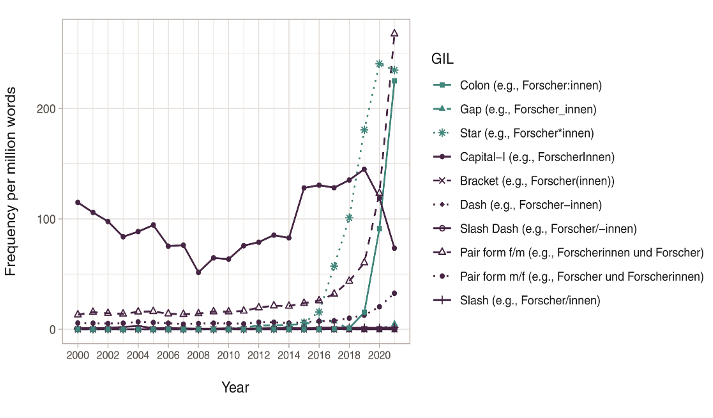
\includegraphics[width=1\textwidth]{gfl_types_frequency.png}
	\caption{Frequency of different types of gender-inclusive language. Source: \citet{waldendorfWordsChangeIncrease2024}.}
	\label{fig:gfl_types_frequency}
\end{figure}


\subsection{English-German Studies}
This language pair in particular is sparsely analysed in academia. I found four relevant papers about gender bias in EN-DE MT that fit my inclusion criteria defined in chapter \ref{subsection:selection_criteria}. Some other sources include German among multiple target languages (e.g. \citeauthor{stanovskyEvaluatingGenderBias2019}'s foundational study), but these do not provide detailed analysis specific to German. Therefore, I do not consider them EN-DE focused sources. The following studies provide a closer look at gender bias specifically in this language pair.

\textbf{\cite{ullmannGenderBiasMachine2022}} performed a corpus-linguistic analysis of training data, meaning they studied large collections of text to identify patterns and structures related to gender bias. The dataset consisted of 17.2 million sentence pairs sourced from \href{https://commoncrawl.org/}{\textit{Common Crawl}}. They then tested different techniques to reduce gender bias in a MT system trained on that corpus. Their findings support the broader patterns discussed in this thesis: masculine forms dominate by default, gender stereotypes shape translations, and professions are translated in line with societal roles. Their key contribution lies in testing mitigation strategies. They show that fine-tuning with a small, gender-balanced dataset can reduce bias in MT outputs. 

\textbf{\citet{rescignoGenderBiasMachine2023}} evaluated gender bias in Google Translate and DeepL for EN-IT and EN-DE using the \href{https://github.com/amazon-science/machine-translation-gender-eval}{MT-GenEval} dataset. They focused on how often professions were translated with male or female forms, both with and without gender-revealing context. Without context, both systems defaulted strongly to masculine forms (over 85\%) for both languages. Contextual information generally improved alignment with reference translations, but in a few cases, context led to incorrect gender disambiguation that had not occurred without it. This suggests that contextual cues can occasionally misguide the system rather than improve performance. The authors also noted that most users are unaware of gender bias, especially if they lack fluency in the source language. Currently there is no system in place to inform them when biased translations occur.

\textbf{\citet{lardelliBuildingBridgesDataset2024}} created a \href{https://github.com/g8a9/building-bridges-gender-fair-german-mt}{Gender-Fair German Dictionary} that includes professions and common nouns for people. They tested several MT systems and evaluated translations from Wikipedia and parliamentary texts. Translations were manually annotated as masculine, feminine, gender-neutral, or gender-inclusive. They also used zero-shot detection with GPT models, where GPT tries to identify gender fairness without specific training. Results showed strong masculine bias and poor automatic detection of GFL, requiring human review and therefore proving zero-shot detection to be challenging. Unlike most research focusing on professions, this study covers a broader range of terms.

\textbf{\citet{kapplAreAllSpanish2025}} introduced \href{https://github.com/michellekappl/mt_gender_german}{WinoMTDE}, a German gender bias evaluation test set based on \citealp{stanovskyEvaluatingGenderBias2019}'s WinoMT. It contains 288 balanced German sentences with clearly gendered subjects and tests occupational stereotyping in MT from German to other gendered languages. The study found that gender bias persists due to model architecture and training data, not source language ambiguity. In experiments, \href{https://openai.com/index/gpt-4o-mini-advancing-cost-efficient-intelligence/}{GPT-4o-mini} performed best overall, while rule-based systems like \href{https://www.systransoft.com/}{SYSTRAN} helped reduce bias in Romance languages but struggled with Slavic and Semitic languages. Major limitations of the study include the small dataset size and broad occupation categories. It also misses some bias types and faces alignment issues affecting accuracy estimates. They call for future researchers to expand the dataset, improve annotations and include diverse gender terms.


\subsection{Cross-Language Perspectives}
Gender bias in MT is not limited to English and German. Many other language pairs show similar patterns, revealing how bias is shaped by both language and the systems behind it. This section includes a few examples from other languages to show that the issue is not specific to German in order to keep the broader context in mind and avoid a narrow, language-specific perspective.

Some studies looked at \textbf{back-translation from English through gender-neutral languages} like Finnish, Indonesian, and Turkish, then back to English. They found different pronoun patterns depending on the language. This shows why it is important to study many languages to understand gender bias better. Verbs played a big role in how gender was inferred in translations. New metrics, like Adjusted Uncertainty, helped capture these details. Some translation systems showed signs of reducing bias over time \citep{barclayInvestigatingMarkersDrivers2024a}.

When translating \textbf{gender-neutral Korean into English}, MT systems often leaned toward masculine pronouns. This happened because the training data had more male examples. Some systems made technical changes that sometimes favored feminine forms, which suggests bias mitigation is possible, however ideally, translations should stay neutral or balanced \citep{choMeasuringGenderBias2019}. \textbf{Japanese and Chinese} demonstrated exceptionally low percentages of female pronouns in translations, going as low as 0.196\% for Japanese and 1.865\% for Chinese \citep{pratesAssessingGenderBias2019}.

Even when translating \textbf{between languages that both use grammatical gender}, like German and Spanish, Ukrainian, or Russian, gender bias still shows up \citep{kapplAreAllSpanish2025}. This goes against the assumption that clear grammatical cues would reduce ambiguity and help systems make better choices. Instead, the bias often stays or even gets worse, suggesting that the problem is not just about language structure but also how MT systems learn and generalize from data.

Most studies focus on English paired with another Western language, with only a few exceptions including West or East Asian languages. This adds an Anglocentric bias to the existing gender bias problem \citep{savoldiDecadeGenderBias2025}.


\section{Mitigation Strategies and Current Limitations}    

In respose to the clear issue of gender bias in NLP, different approaches have been tested to mitigate it.

NOTE THAT I AM NOT LOOKING AT MITIGATING IT IN A GENERAL SENSE DUE TO THE SHEER DIFFICULTY OF IT. THE FIRST STEP IS DETECTING SINCE THERE ARE FEW DETECTION SYSTEMS THAT COULD PROVIDE A BASE FIRST. I DONT AIM TO DEBIAS I AM TO RAISE AWARENESS. ZERO SHOT HAS MOSTLY FAILED WITH LLMS SO I WANT TO SEE HOW WELL FINE TUNING PERFORMS.

% ullmann

% Mitigating Gender Bias:
% ◦
% While removing all bias is practically impossible and a completely bias-free dataset might misrepresent society, strategies can be deployed at different stages.
% ◦
% Pre-training Techniques:
% ▪
% Downsampling: Removing data until gendered terms are balanced.
% ▪
% Upsampling: Duplicating data to achieve a balanced ratio.
% ▪
% Counterfactual Augmentation: Introducing new sentences that include under-represented gendered terms (e.g., adding "She is a doctor" if only "He is a doctor" exists).
% ▪
% Results: These pre-training techniques showed no notable gains in accuracy compared to existing systems; counterfactual augmentation performed best but was still worse than other systems.
% ◦
% Post-training Technique (Fine-tuning):
% ▪
% Ullmann's research demonstrated that significantly less biased output could be achieved by fine-tuning an MT system, after its initial training, with a small, gender-balanced dataset. This involved a dataset of 388 sentence pairs based on 194 professions.
% ▪
% Conclusion: This "model adaptation" is a practical partial solution to gender bias in MT.

Technical Approaches:

Fine-tuning models with balanced data 9

Context-aware architectures 11

Gender-neutral translation strategies 9

LLM Potential: While promising, current LLMs like ChatGPT often introduce new biases when explicitly prompted for gender alternatives 9.

Persistent Challenges:

English-centric approaches dominating research 4

Disconnect between translation technologies and operational contexts 4

Difficulty handling non-binary identities

\section{Positioning of My Work}    
% - How your work builds on these findings.
% - What gap you address (binary classifier + demo).
    
%     **Use:** Comparison with prior methods.